% This is the Duke University Statistical Science LaTeX thesis template.
% It has been adapted from the Reed College LaTeX thesis template. The
% adaptation was done by Mine Cetinkaya-Rundel (MCR). Some of the comments
% that are specific to Reed College have been removed.
%
% Most of the work on the original Reed College document class and template
% was done by Sam Noble (SN). Later comments etc. by Ben Salzberg (BTS).
% Additional restructuring and APA support by Jess Youngberg (JY).
%
% See https://www.reed.edu/cis/help/latex/ for help. There are a
% great bunch of help pages there, with notes on
% getting started, bibtex, etc. Go there and read it if you're not
% already familiar with LaTeX.
%
% Any line that starts with a percent symbol is a comment.
% They won't show up in the document, and are useful for notes
% to yourself and explaining commands.
% Commenting also removes a line from the document;
% very handy for troubleshooting problems. -BTS

%%
%% Preamble
%%
% \documentclass{<something>} must begin each LaTeX document
\documentclass[12pt,twoside]{dukestatscithesis}
% Packages are extensions to the basic LaTeX functions. Whatever you
% want to typeset, there is probably a package out there for it.
% Chemistry (chemtex), screenplays, you name it.
% Check out CTAN to see: http://www.ctan.org/
%%
\usepackage{graphicx,latexsym}
\usepackage{amsmath}
\usepackage{amssymb,amsthm}
\usepackage{longtable,booktabs,setspace}
\usepackage{chemarr} %% Useful for one reaction arrow, useless if you're not a chem major
\usepackage[hyphens]{url}
% Added by CII
\usepackage{hyperref}
\usepackage{lmodern}
\usepackage{float}
\floatplacement{figure}{H}
% End of CII addition
\usepackage{rotating}

% Next line commented out by CII
%%% \usepackage{natbib}
% Comment out the natbib line above and uncomment the following two lines to use the new
% biblatex-chicago style, for Chicago A. Also make some changes at the end where the
% bibliography is included.
%\usepackage{biblatex-chicago}
%\bibliography{thesis}


% Added by CII (Thanks, Hadley!)
% Use ref for internal links
\renewcommand{\hyperref}[2][???]{\autoref{#1}}
\def\chapterautorefname{Chapter}
\def\sectionautorefname{Section}
\def\subsectionautorefname{Subsection}
% End of CII addition

% Added by CII
\usepackage{caption}
\captionsetup{width=5in}
% End of CII addition

% \usepackage{times} % other fonts are available like times, bookman, charter, palatino


% To pass between YAML and LaTeX the dollar signs are added by CII
\title{Stochastic Process Model with Basketball Data}
\author{Sonia Xu}
% The month and year that you submit your FINAL draft TO THE LIBRARY (May or December)
\date{October 2017}
\advisor{Dr.~Alexander Volfovsky}
\institution{Duke University}
\degree{Bachelor of Science in Statistical Science}
\committeememberone{Committeemember O. Name}
\committeemembertwo{Committeemember T. Name}
\dus{Dus X. Name}
%If you have two advisors for some reason, you can use the following
% Uncommented out by CII
% End of CII addition

%%% Remember to use the correct department!
\department{Department of Statistical Science}

% Added by CII
%%% Copied from knitr
%% maxwidth is the original width if it's less than linewidth
%% otherwise use linewidth (to make sure the graphics do not exceed the margin)
\makeatletter
\def\maxwidth{ %
  \ifdim\Gin@nat@width>\linewidth
    \linewidth
  \else
    \Gin@nat@width
  \fi
}
\makeatother

\renewcommand{\contentsname}{Table of Contents}
% End of CII addition

\setlength{\parskip}{0pt}

% Added by CII

\providecommand{\tightlist}{%
  \setlength{\itemsep}{0pt}\setlength{\parskip}{0pt}}

\Acknowledgements{
I want to thank a few people.
}

\Dedication{
You can have a dedication here if you wish.
}

\Preface{
This is an example of a thesis setup to use the reed thesis document
class (for LaTeX) and the R bookdown package, in general.
}

\Abstract{
The preface pretty much says it all. \par

Second paragraph of abstract starts here.
}

% End of CII addition
%%
%% End Preamble
%%
%

\usepackage{amsthm}
\newtheorem{theorem}{Theorem}[chapter]
\newtheorem{lemma}{Lemma}[chapter]
\theoremstyle{definition}
\newtheorem{definition}{Definition}[chapter]
\newtheorem{corollary}{Corollary}[chapter]
\newtheorem{proposition}{Proposition}[chapter]
\theoremstyle{definition}
\newtheorem{example}{Example}[chapter]
\theoremstyle{definition}
\newtheorem{exercise}{Exercise}[chapter]
\theoremstyle{remark}
\newtheorem*{remark}{Remark}
\newtheorem*{solution}{Solution}
\begin{document}

% Everything below added by CII
  \maketitle

\frontmatter % this stuff will be roman-numbered
\pagestyle{empty} % this removes page numbers from the frontmatter
  \begin{acknowledgements}
    I want to thank a few people.
  \end{acknowledgements}
  \begin{preface}
    This is an example of a thesis setup to use the reed thesis document
    class (for LaTeX) and the R bookdown package, in general.
  \end{preface}
  \hypersetup{linkcolor=black}
  \setcounter{tocdepth}{2}
  \tableofcontents

  \listoftables

  \listoffigures
  \begin{abstract}
    The preface pretty much says it all. \par
    
    Second paragraph of abstract starts here.
  \end{abstract}
  \begin{dedication}
    You can have a dedication here if you wish.
  \end{dedication}
\mainmatter % here the regular arabic numbering starts
\pagestyle{fancyplain} % turns page numbering back on

\chapter{thesisdowndss::thesis\_gitbook:
default}\label{thesisdowndssthesis_gitbook-default}

\chapter{Placeholder}\label{placeholder}

\chapter{Literature Review}\label{rmd-basics}

Passing forms the backbone of all team contact sports. To advance a ball
to the goal successfully, players must work together to
dribble/kick/throw the ball to its destination. Each pass to another
player can be considered a connection. These connections can be grouped
together to form a network of passes. Previous works have captured these
passing networks in soccer and basketball both statically and
dynamically--this literature review will explore the different methods
used to understand the value of a player and team.

``Flow Motifs in Soccer: What can passing behavior tell us?'' by Joris
Bekkers and Shaunak Dabadghao was released in the 2017 MIT Sloan Sports
Analytics Conference, and focused on the static passing networks of
``the last 4 seasons of 6 big European leagues with 8219 matches, 3532
unique players and 155 unique teams.'' Passing sequences were denoted as
a sequence of all players involved five seconds before an attempted
score. This paper created radar graphs that illustrated the most popular
passing sequences by player, and compared radar graphs to identify
similar players. Passing sequences within teams were also compared
between teams by clustering the different passing styles of the
different teams. Key players were determined by the frequency that they
were included in the passing sequences.

``Exploring Team Passing Networks and Player Movement Dynamics in Youth
Association Football (Soccer)'' by Bruno Goncalves, Diogo Coutinho, Sara
Santos, Carlos Lago-Penas, Sergio Jimenez, and Jamie Sampaio compared
the passing sequences of two games played by two groups that differ in
age range, which showed that regardless of age, network centrality was
distinctive in both groups, and affirmed the long-held belief that more
passes lead to better game outcomes. Similar to the first paper, key
players were the ones most frequently involved in the passing sequences.
This paper created weighted graphs of the passing sequences, which
better visualized the passing structure of the team, and made it easier
to identify important players.

``Basketball Teams as Strategic Networks'' by Jennifer H. Fewell, Dieter
Armbruster, John Ingraham, Alexander Petersen, and James S. Waters
provided measurements to assess team entropy. First recording the
complete 30 seconds of a possession as a passing sequence, they
discovered that recording the last three nodes (players) before a shot
attempt was a better way to record passing sequences to avoid ``noisy''
passing data. Although they were able to recognize various aspects of
team dynamics through weighted graphs like the second paper, they did
not find a consistent predictor of positive game outcomes. This paper
also identified that in general, teams typically range between two
playing styles: always passing to the best player or having no distinct
patterns in passing. These patterns can be noted by distinct betweenness
scores and uniform betweenness scores, respectively. Weighted graphs
clearly illustrated the two different playing styles. Also, the paper
found that the positions most involved with successful shots were: 1. PG
2. SG 3. SF 4. PF 5. CN.

Joachim Gudmundsson and Michael Horton summarised a variety of methods
that utilize object tracking data to analyze team and player
performances in ``Spatio-Temporal Analysis of Team Sports -- A Survey.''
Their research survey spanned modeling passing networks via graph theory
to calculating rebound probability with spatial coordinates. In
particular, work conducted by Daniel Cervone, Alex D'Amour, Luke Bornn,
and Kirk Goldsberry attempted to capture the game wholelistically via a
new measure called Expected Possession Value (EPV) in the paper ``A
Multiresolution Stochastic Process Model for Predicting Basketball
Possession Outcomes.'' This new metric uses three models--a
Microtransition Model, Macrotransition Entrance Model, and a
Macrotransition Exit Model--to capture the spatial biases of each player
and the in-game effects of pressure, so that it can measure the
likelihood of a successful play (made shot) given the previous sequence
of events. To compare players against the league-average scores, they
also calculated Expected Possession Value -Adjusted as an application
for teams.

\chapter{Dataset}\label{dataset}

The dataset is from the Duke University Men's Basketball SportsVu
tracking data. Features were created by taking snapshots of the game
every 1/25th of a second and recording the player's location, action,
team, etc. Data was collected for each season from 2013-2016; the
dataset totals about 2 million observations and 72 features.

\chapter{Model Replication}\label{model-replication}

The initial approach to understand how to best capture passing networks
sought to replicate Daniel Cervone, Alex, D'Amour, Luke Bornn, and Kirk
Goldsberry's paper,``A Multiresolution Stochastic Process Model for
Predicting Basketball Possession Outcomes.'' They attempt to capture the
game wholelistically via a new measure called Expected Possession Value
(EPV). This new metric uses three models--a Microtransition Model,
Macrotransition Entrance Model, and a Macrotransition Exit Model--to
capture the spatial biases of each player and the in-game effects of
pressure, so that it can measure the likelihood of a successful play
(made shot) given the previous sequence of events. To compare players
against the league-average scores, they also calculated Expected
Possession Value -Adjusted as an application for teams. Below is a brief
overview of each model.

This paper is particularly interesting because EPV utilizes the
spatio-temporal elements of the game, so it models the NBA game
dynamically. Given Duke Basketball data, the motivation is to replicate
``A Multiresolution Stochastic Process Model for Predicting Basketball
Possession Outcomes,'' to better understand the Duke Men's team, as well
as to compare professional basketball to collegiate basketball
individual and team playing styles. Below is a brief overview of each
model used in the paper to calculate EPV.

\section{Microtransition Model}\label{microtransition-model}

\(x^{l}(t+\epsilon) = x^{l}(t) + \alpha^{l}_{x}[x^{l}(t) - x^{l}(t-\epsilon)] + \eta^{l}_{x}(t)\)
where
\(\eta^{l}_{x}(t) \sim N(\mu^{l}_{x}(z^{l}(t)), (\sigma^{l}_{x})^{2})\)

The microtransition model models the defensive conditions of the game
based on the \((x,y)\) coordinates of a player and their acceleration
effects (\(\alpha^{l}_{x}(t)\)). It is also assumed that a player's
spatial location is normally distributed. Since players play
differently, each microtransition model is specifically fitted to the
player.

\section{Macrotransition Entrance
Model}\label{macrotransition-entrance-model}

\(P(M(t)|F_{t}^{(Z)}\) The macrotransition entrance model predicts
whether the next move will be a pass (4 options), shot attempt, or
turnover. The model is disjoint.

\section{Macrotransition Exit Model}\label{macrotransition-exit-model}

\(P(C_{\delta_{t}}|M(t), F_{t}^{(Z)})\) Given the Macrotransition
Entrance Model predicts a shot attempt, it indexes to a logistic
regression model to calculate player \(l\)'s successful shot
probability. Given the Macrotransition Entrance Model predicts a pass,it
indexes to a model that predicts where the pass will take place.
Otherwise, a turnover is assumed.

\section{Fall Backs on the Implementation of this
Model}\label{fall-backs-on-the-implementation-of-this-model}

\section{in the works\ldots{}}\label{in-the-works}

\section{Next Steps (have yet to get this
far)}\label{next-steps-have-yet-to-get-this-far}

Both metrics calculated via a semi-Markov process, EPV fails to capture
the full nature of the possession because it only uses the last
posession as a prior. The model would be more robust if it captured the
entirety of the posession in its prior--however, the computational time
of such an ordeal would prevent any real-time analyses. Thus, this paper
proposes that a simpler model may perform more quickly and potentially
just as robustly to allow for game-time analyses.

\chapter{Exploratory Data Analysis}\label{exploratory-data-analysis}

\section{Changes in Shot Attempt
Patterns}\label{changes-in-shot-attempt-patterns}

As one of the best basketball programs in the nation, Duke University
Men's Basketball draws in a number of highly desirable and NBA-ready
recruits each year. For this, most players stay for only a year before
signing and playing for the National Basketball Association. A popular
trend for many skilled basketball players, this transition to
professional basketball has been coined by players as being
``one-and-done.'' Duke had two players (Rodney Hood, Jabari Parker)
drafted in the 2014 draft, three players (Jahlil Okafor, Justise
Winslow, and Tyus Jones) drafted in the 2015 draft, and one player
(Brandon Ingram) drafted in the 2016 draft. With so many players playing
the minimum in college, this paper concentrates on the analysis of
players who played more than one season with the Duke Men's Basketball
team, and had significant minutes with their time at Duke. With these
requirements, it is difficult to find the perfect player for analysis
because players like Marshall Plumlee, only had significant playing time
his senior year because it took time to fully develop him as a
competitive player.

Quinn Cook, on the other hand, serves as an interesting example because
he had consistent minutes for the 2013-2015 seasons. Quinn Cook's shot
attempts were thus divided into each year to understand how his shooting
style has changed during his time at Duke.
\begin{figure}
\centering
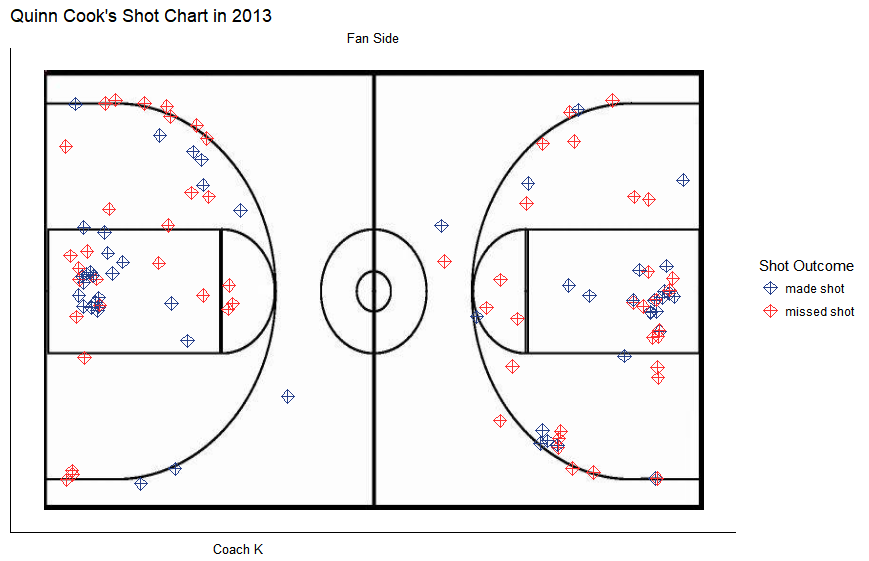
\includegraphics{img/shotchart_quinncook2013.png}
\caption{}
\end{figure}
Looking at the Quinn Cook's shot attempts for his junior season, he was
fairly even with his shooting, missing most of his 3 point shots, and
hitting most of his 2 point shots in the paint. It appears as though he
prefers to shoot from the left wing slightly more than he shoots from
the right wing.
\begin{figure}
\centering
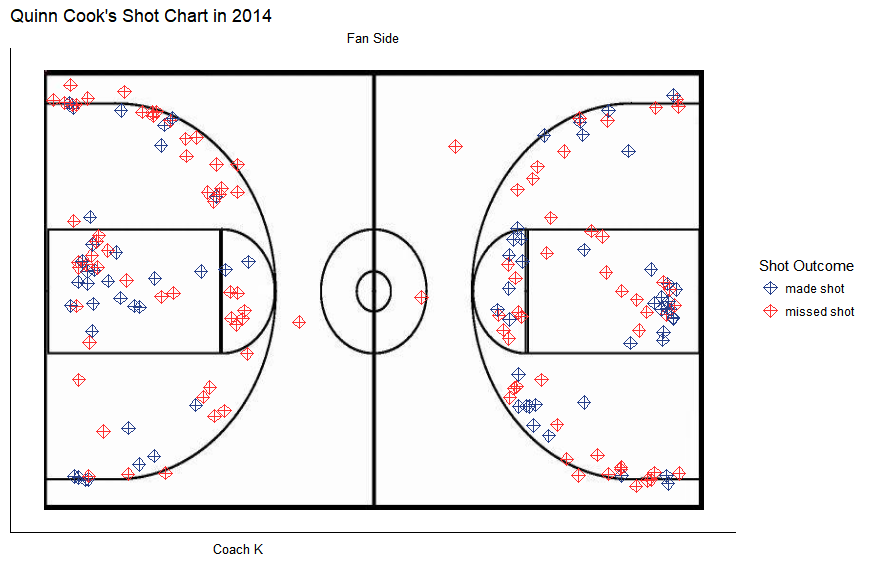
\includegraphics{img/shotchart_quinncook2014.png}
\caption{}
\end{figure}
In 2014, however, it can be noted that Quinn Cook has transitioned to
shots that are closer to the basket and minimized the amount of 3 point
shot attempts. He brought his shot attempts closer inwards, which aligns
with the trend that he is better at shooting when he is closer to the
basket. Compared to 2013, he attacks more along the nail, which could be
attributed to Quinn Cook's growing strength as an off-the-jump shooter.
\begin{figure}
\centering
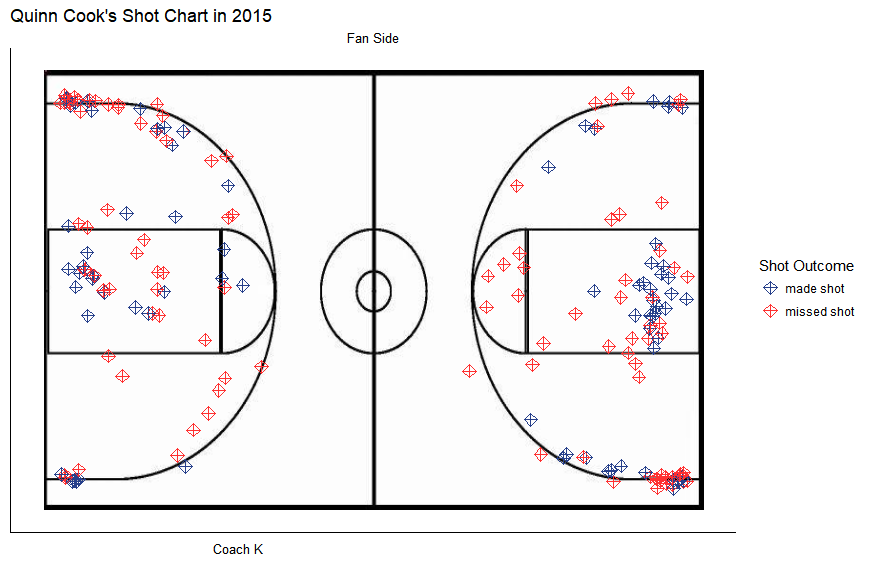
\includegraphics{img/shotchart_quinncook2015.png}
\caption{}
\end{figure}
In the 2015 season, Quinn Cook moves further out from the basketball,
attempting more 3s. His preference for shooting in the left wing is more
pronounced. A new trend apparent from the graph, however, shows that
Quinn Cook shoots more corner 3s than the previous two years. While his
shot attempts in the paint have slightly changed from 2013, Quinn Cook
definitely has a unique playing style that has overall been consistent
in that he avoids shooting in the extended elbows and short corners.

\section{Biases in Shot Location}\label{biases-in-shot-location}

Based off of the

\section{Networks}\label{networks}
\begin{figure}
\centering
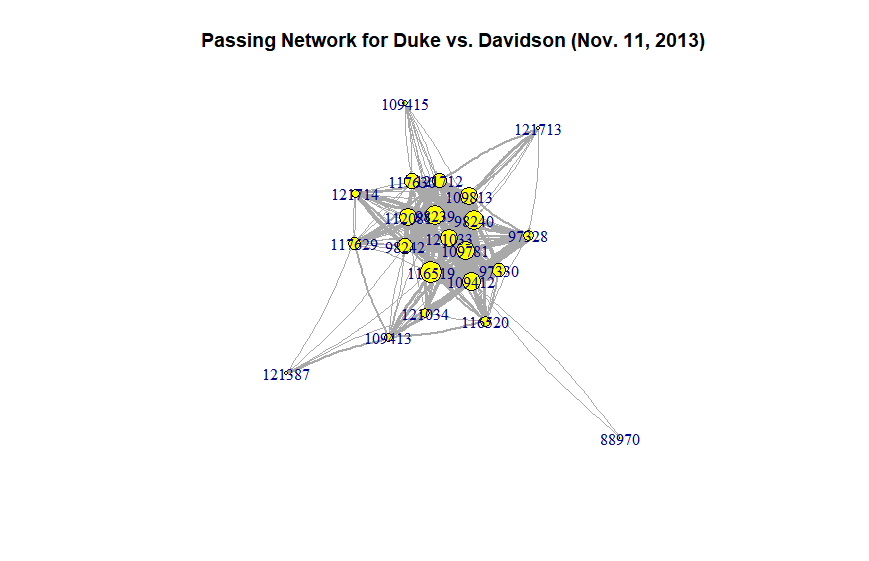
\includegraphics{img/gamenetwork_ex.png}
\caption{}
\end{figure}
\chapter{This chunk ensures that the thesisdowndss package
is}\label{this-chunk-ensures-that-the-thesisdowndss-package-is}

\chapter{Organization}\label{organization}

\chapter*{Conclusion}\label{conclusion}
\addcontentsline{toc}{chapter}{Conclusion}

\chapter{The First Appendix}\label{the-first-appendix}

\chapter*{References}\label{references}
\addcontentsline{toc}{chapter}{References}


% Index?

\end{document}
